\chapter{Discussion}

\begin{center}
    \textit{The results are analyzed and discussed in this chapter. It explores the implications of the findings, identifies limitations, and suggests potential areas for future improvement.}
\end{center}

\section{Overview of Delivered Product}
The delivered product functions as intended and meets all defined requirements. It allows players to conduct \gls{otb} chess games using a traditional physical board, while each move is automatically detected, validated, and stored digitally in \gls{pgn} format. These \gls{pgn} files can be accessed in real time through the frontend interface, enabling both live viewing and post-game analysis. \\

The core functionality of the system has proven to be reliable across different test scenarios, see section \ref{machine-learning-test}. Players are able to engage with the game naturally, without needing to alter their usual playing behavior or interact directly with the system during game play. The seamless digitization process provides a user-friendly experience, especially for tournament organizers or spectators who wish to follow games live. \\

Despite this, a minor delay is present between the moment a physical move is made and its appearance on the digital board. This latency is primarily caused by the time required for image capture, model inference, and subsequent processing. While the delay does not significantly impact usability, it could be minimized through further optimization of the machine learning models or by deploying the system on more powerful hardware. \\

Move validation is handled through a three-step process to ensure both accuracy and legality of each detected move. The machine learning model first detects changes on the board, followed by backend validation using a chess engine that checks the move against the current game state. Finally, the frontend performs an additional check before updating the display. If an illegal move is identified at any point, the system stops further updates to prevent errors or corrupted game data. In line with the product owner's request, the system includes no extra error handling or user notifications. It is intended solely as a display tool for passive observation and live broadcasting, not as an active referee. This approach keeps the interface simple while preserving reliable and consistent game visualization.

\section{Machine Learning Model}

The overall move accuracy across all games was 90.6\%. Performance between board types was similar, with slightly better detection rates on the wooden board (91.2\%) compared to the plastic board (89.9\%), as shown in Table~\ref{tab:board-type-accuracy}. This minor difference may be attributed to the higher visual contrast between the wooden pieces and the board surface, than the black and white pieces for the plastic board. \\

While the ChessCam models used in this project demonstrate high precision and recall under ideal conditions (Section \ref{chesscam-metrics}), our real-world move detection accuracy of 90.6\% is naturally lower. This is expected, as full move detection in physical games involves not just accurate identification of pieces and board geometry, but also handling lighting variations, ambiguous moves (castling) and general noise. Thus, the ChessCam metrics serve more as an upper bound, while our results reflect the practical challenges of real-time, physical chess move recognition. \\

One consistent source of error was tied to specific move numbers within certain openings. In some test sets, all 10 games of a particular opening failed at the same move, suggesting that specific board states challenge the model. This caused some piece types, especially the black rook, to receive unusually low scores (23.8\%). Since black rooks had relatively few moves overall and repeatedly failed at the same point in the games, their scores were artificially suppressed. \\

Another common issue involved the model misclassifying castling moves. The model selects the move with the highest predicted probability, but during castling, it often assigned a higher probability to the rook’s move from its original square rather than to the king’s two-square move. As a result, castling was frequently mistaken for a rook move. Of the 9 total misclassifications, 8 were caused by this specific error. One potential solution is to delay the rook’s movement by moving the king two squares first. This would give the model only one valid move to detect, reducing the likelihood of misclassification. \\

We also observed reduced accuracy along the edges of the board, affecting both piece detection and the localization of square centers. Several factors contribute to this. The board-warping algorithm depends heavily on precise corner detection, which is more error-prone near the edges. The steep camera angle causes pieces closer to the camera to appear larger and obscure important details. Meanwhile, pieces farther away appear smaller and are more difficult to detect. Figure~\ref{fig:bbox-centers-incorrect} illustrates this issue, showing bounding boxes near the edges that are frequently misaligned and square centers that are noticeably offset. In contrast, detection accuracy and alignment improve significantly toward the center of the board.

Another limitation observed was the model's handling of the en passant. Currently, the model does not support recognition of en passant moves. When the board state includes the possibility for such a move, the model fails to handle it correctly and crashes.


\begin{figure}[h!]
    \centering
    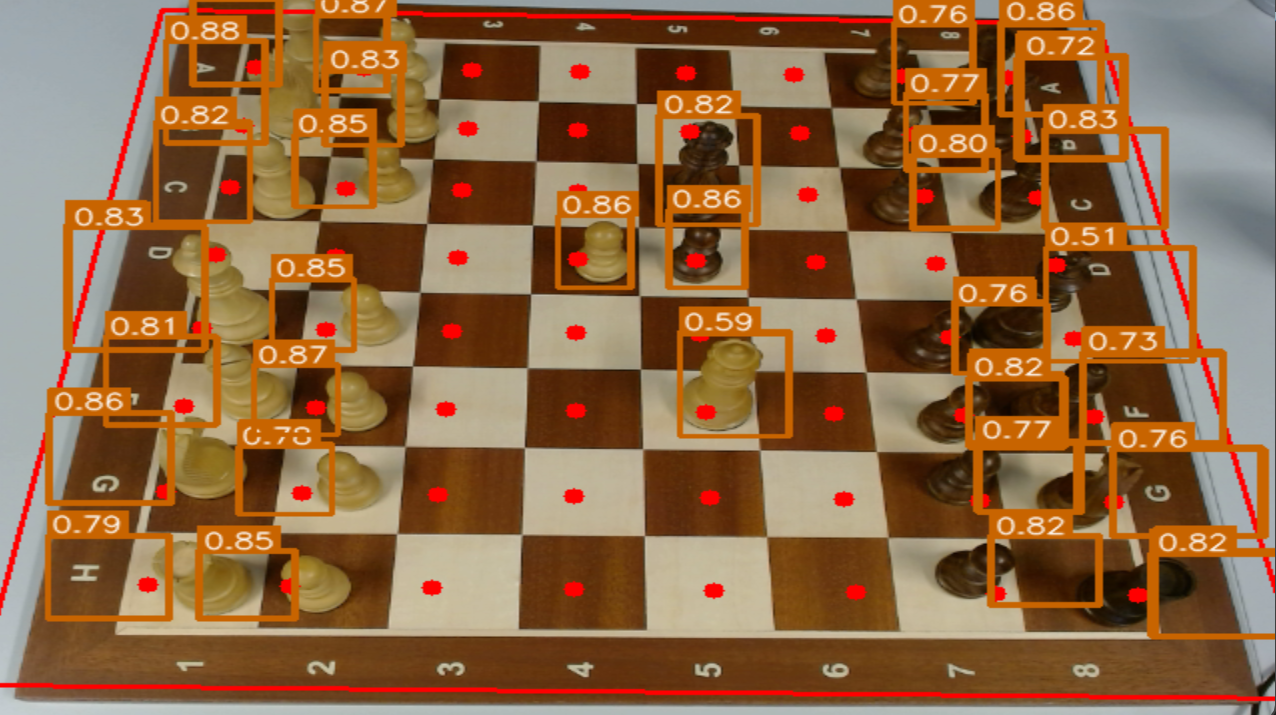
\includegraphics[width=0.75\linewidth]{figures/discussion/bbox-centers-incorrect.png}
    \caption[Bounding box and square center misalignment]{Bounding boxes and square centers overlaid on a physical chessboard. Boxes and square centers near the edges are misaligned.}
    \label{fig:bbox-centers-incorrect}
\end{figure}


\section{API}
The system follows a client-server architecture, where the frontend acts as the client and communicates with a centralized backend server responsible for handling data processing and move validation. This separation ensures a scalable and maintainable structure, allowing each part of the system to operate independently while still interacting efficiently. To enable real-time communication between the components, the WebSocket protocol was used. Unlike traditional HTTP, which relies on a request-response cycle, WebSocket maintains a persistent connection that allows data to be sent and received continuously. This approach reduces latency and network load by eliminating the need for constant polling, ensuring that the frontend receives updates as soon as new moves are processed by the backend.

\section{Frontend}
The frontend was developed based on the initial wireframes but was modified throughout the project in response to feedback from the supervisor, product owner, and user testing. Despite these adjustments, the core components and functionality remained consistent with the original design.

\subsection{Game preview}
The Game Preview page was not part of the initial wireframe, as described in Section \ref{subsec:wireframe}. However, following a suggestion from the product owner, this feature was added to provide a better overall overview of all ongoing games. One scenario for this functionality is when a spectator wishes to follow multiple games simultaneously. \\

Since the application architecture was already based on individual chessboard instances, implementing this feature was relatively straightforward. By reusing existing chessboard components identified by unique IDs, the Game Preview page was able to display all active games dynamically. Only minor code modifications were necessary to make the component more flexible and support this functionality.

\subsection{Download PGN file}
One project requirement was to digitize chess games into \gls{pgn} files, enabling players and spectators to download and analyze them using external tools such as \gls{lichess}’ analysis feature. As described in Section~\ref{subsec:results-frontend}, the application provides access to PGN files containing technical metadata. \\

The \gls{pgn} format is widely supported, and tools such as \gls{lichess} can interpret both the complete file or just the move list. This flexibility allows users to gain insights into various aspects of the game, such as identifying the opening played, evaluating move accuracy, and understanding the overall game progression. Figure~\ref{fig:downloaded-pgn-analysis} shows how the downloaded \gls{pgn} can be used in an external analysis tool. \\

\begin{figure}[h!] \centering \fbox{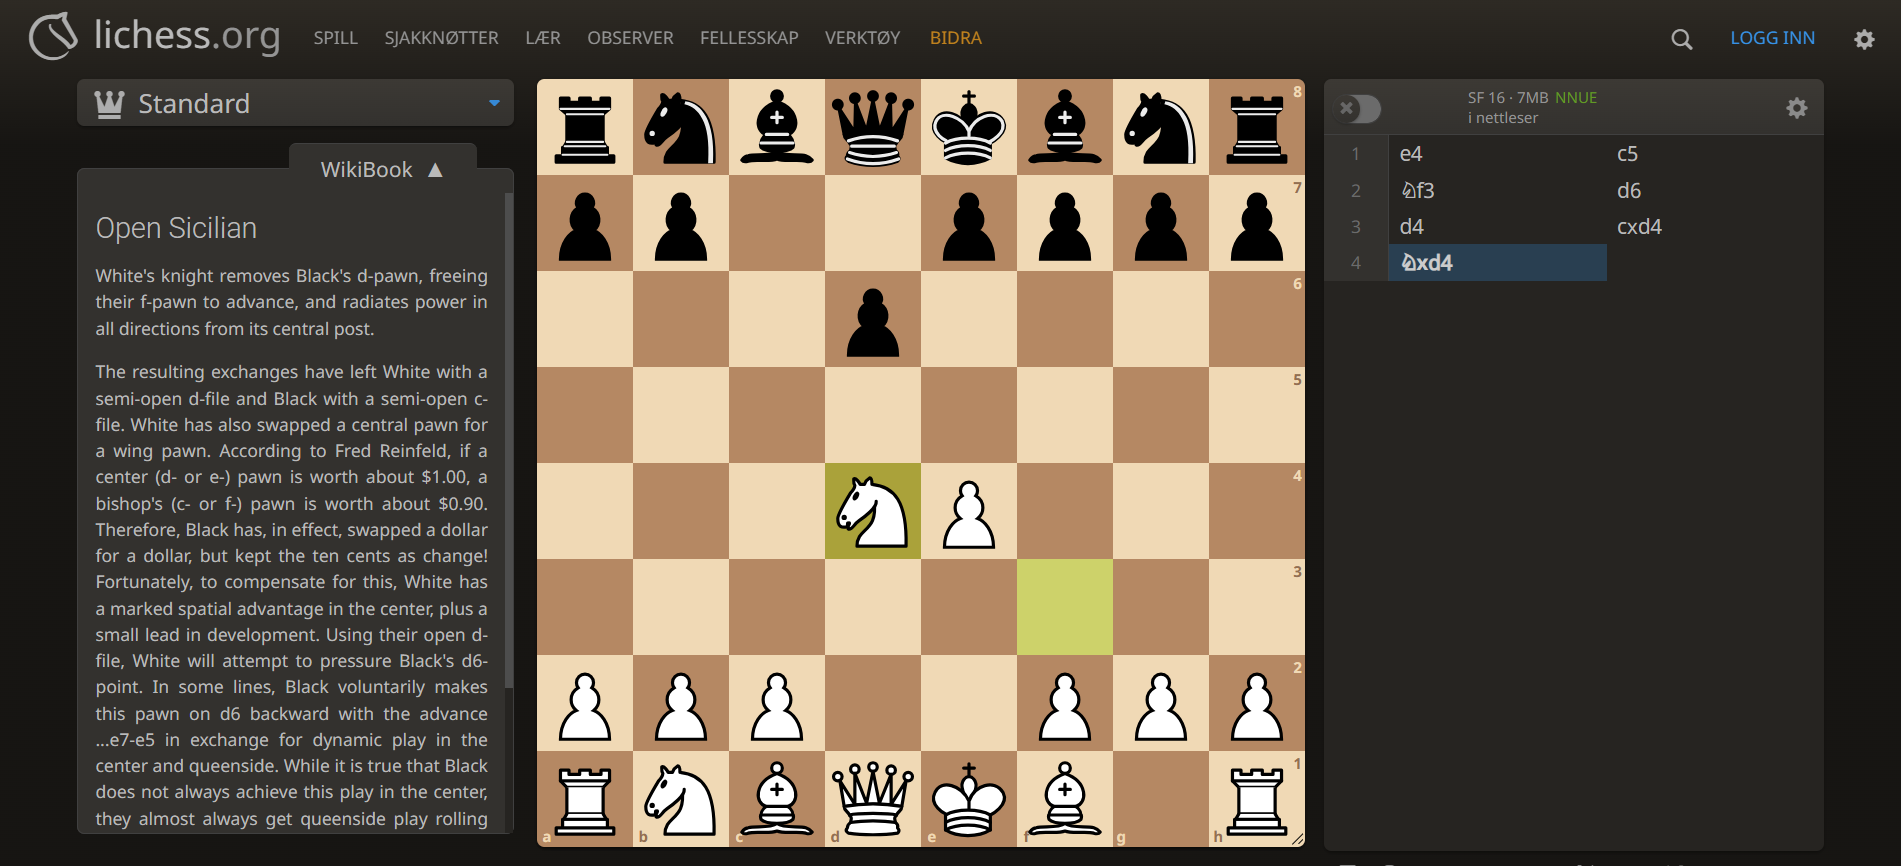
\includegraphics[width=0.75\linewidth]{figures/results/frontend/download-pgn/lichess-analysis.png}}\caption[Lichess analysis tool]{A demonstration of importing a PGN file into Lichess' analysis tool}\label{fig:downloaded-pgn-analysis} \end{figure}

By enabling \gls{pgn} downloads, the system provides users with a convenient way to review games and improve their understanding of chess. Instead of building a custom in-app analysis feature, this solution leverages existing, well-established services that offer robust and detailed feedback. This decision reduces development complexity while still providing users with valuable insights. \\

However, one limitation is that users must leave the application to analyze the game, which can disrupt the user experience. Despite this, integrating \gls{pgn} downloads remains a practical and effective solution, offering immediate access to game data without requiring additional implementation of complex analytical features.

\subsection{Lighthouse Tests}
The frontend application was developed based on wireframes, team discussions, and user testing. To evaluate the quality of the user interface, Lighthouse tests were conducted on every page, with particular focus on the accessibility score. \\

Initial accessibility scores ranged from 80 to 90 across the various pages. To improve these scores, several adjustments were required—primarily involving color contrast. As shown in \ref{subsec:results-color-palette}, a specific color palette was selected for the application. However, issues were identified with the contrast between the primary blue color and the white background in light mode, as well as between the secondary blue (used for buttons) and the black background in dark mode. \\

To address these issues, slightly modified color variants were chosen for each theme. This led to the adoption of a more customized color palette for both light and dark modes. As a result, the application now achieves a 100 accessibility scores throughout all pages, with both light and dark mode. 

\section{Project management}
\label{sec:discussion-project-management}

The application of a Scrum inspired methodology proved to be an effective project management strategy, particularly given the composition and size of the team. While the team followed core Scrum practices such as sprint planning, reviews, and retrospectives, the absence of a dedicated Scrum Master led to a more lightweight and adaptive implementation. Responsibilities typically associated with the Scrum Master role, such as facilitating meetings and managing the sprint process, were informally distributed among team members. This approach enabled greater flexibility and autonomy, which aligned well with the needs of a smaller team. \\

The communication within the team functioned efficiently throughout the project. Daily in-person collaboration during office hours allowed for rapid feedback, informal stand-ups, and immediate resolution of issues. The accessibility of all team members facilitated a high degree of responsiveness, reducing reliance on scheduled meetings and improving overall coordination.\\

Version control and task management were handled using Git, which provided a robust framework for organizing and reviewing code. Each task was implemented in a dedicated branch and linked to a corresponding GitHub issue. All changes were integrated into the main branch exclusively through pull requests, with peer review enforced for every contribution. This workflow contributed to maintaining code quality, minimizing integration issues, and ensuring transparency in the development process. \\

GitHub Actions was used to automate the development process, including running Python unit tests and updating LaTeX documentation. This improved efficiency and helped catch issues early. However, the test workflow consistently failed in the CI environment due to its dependence on camera hardware (see Figure~\ref{fig:workflow-test}). Since this hardware was unavailable during automated runs, the failures were expected and did not impact the final delivery. This highlighted the need to separate hardware-dependent tests from those suitable for standard test environments.\\

\begin{figure}[h!] \centering 
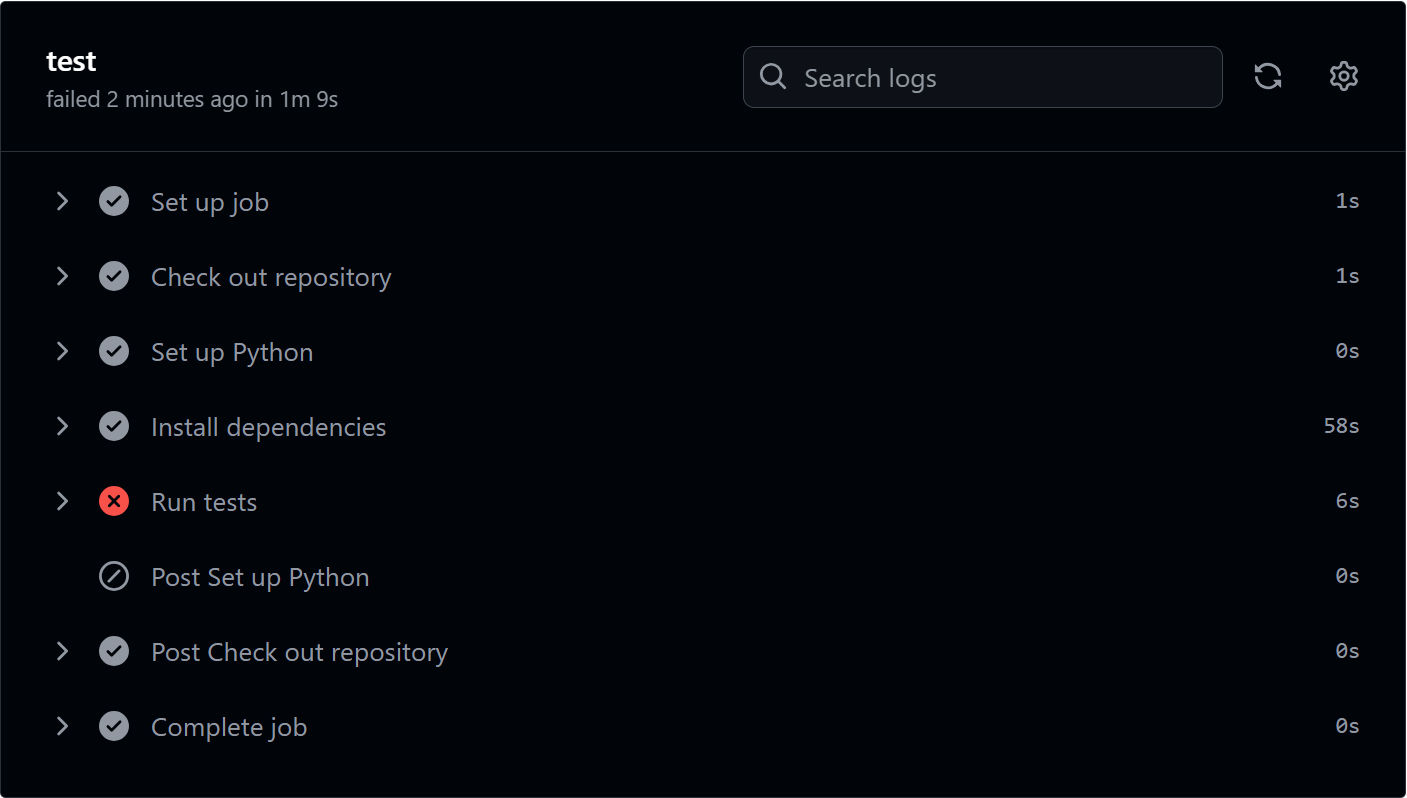
\includegraphics[width=0.75\linewidth]{figures/results/workflows/tests.png}\caption[Python tests workflow]{The workflow for Python unit tests}\label{fig:workflow-test} \end{figure}

Overall, the project management approach successfully balanced structure and flexibility. The adapted Scrum practices, supported by reliable tooling, effective peer review, and strong communication, created a productive environment well-suited to the team's working style. 

\section{Challenges}
In addition to ideas for future development, there were also a few obstacles encountered during development. These challenges were addressed as they occurred, and solutions were implemented as part of the final application. \\

\subsection{Camera}

During development, the application occasionally selected the system’s built-in front camera instead of the intended external USB cameras. The root cause was identified as cached “ghost” devices in the Windows Device Manager. These are records of previously connected hardware that remain stored even after the devices are disconnected. Such ghost entries can cause conflicts and incorrect device indexing, especially when multiple identical cameras are involved, leading to the misassignment of camera IDs. Temporarily, disconnecting the external cameras and restarting the system forced ID reassignment and resolved the problem, though this is not an ideal solution. \\










\subsection{Highlighting moves}
When a move is made, the frontend highlights the previous and current tiles of the moved piece. User testing with different color palettes resulted in the selection of a bright contrast color relative to the main design scheme to ensure good visibility. \\

The chessboard component manages the rules of chess, while the frontend is responsible only for storing tile positions and applying styling. In standard moves, highlighting the starting and ending tiles is sufficient. However, special moves such as \gls{castling}, pawn \gls{promotion}, and \gls{en-passant} capture require additional handling. \\

In \gls{castling}, both the king and a rook move simultaneously. Since the default highlight logic tracks only one piece, it does not correctly represent \gls{castling} moves. Additional logic was implemented to highlight the movements of both the king and rook during \gls{castling}, ensuring consistency and clarity for the user.


% Ting som nevnes andre steder i dokumentet som er flyttet hit fordi det funker bedre i diskusjon


%The ONNX format was chosen because it was framework-agnostic, making integration into different deployment environments easier.

%(Metode, User-Centered Design)

%This encouraged honest, unfiltered responses, reducing the likelihood of social desirability bias.

\section{Further Development}
Throughout the project, various development ideas emerged from the team, the product owner, and external contributors. Due to time constraints, these were not implemented and were instead noted as "Further development." At the product owner's request, the focus was on achieving accurate piece recognition over additional features.

\subsection{Independent Application}
During a meeting at Aalesund Schaklag, the product owner and club leader discussed deploying a finalized version of the application with ceiling-mounted cameras. Since the club maintains a standard table layout, the cameras could remain fixed and connected to a computer running the application continuously. A physical switch would allow easy power control. \\

In a typical use case, the organizer could start an unofficial tournament by turning on the switch, prompting the system to begin tracking games automatically. Once games were finished, the organizer would reset the returned to their initial position would be recognized as reset. The system would be user-friendly, requiring no technical knowledge and would also protect equipment by having cameras out of reach.

\subsection{Information About Participants}
Currently, all tournament participants are hardcoded into the system. This approach limits scalability and increases the complexity of system maintenance. A more sustainable solution would involve integrating the system with established platforms such as TournamentService, a widely used tool for managing player registration in chess tournaments. \\

TournamentService retrieves player data from both the Norwegian Chess Federation (NSF) and the international \gls{fide} database, ensuring that participant information is accurate and up-to-date.
By implementing such an integration, participants would be able to register by simply searching for their name. The system could then automatically retrieve and populate essential details, such as chess rating, club affiliation, and other relevant metadata. This would significantly streamline the registration process and reduce the likelihood of manual entry errors. \\


\subsection{Time Control}
In chess tournaments, different time formats such as \gls{classical}, \gls{rapid}, and \gls{blitz} are commonly used. The current application does not show time control information, making it harder for spectators to follow the games. Displaying the time control format and countdown timer could enhance the spectator experience. \\

One potential solution is to estimate the remaining time based on move detection. When the machine learning model registers a move, it assumes the player has pressed the clock and that the opponent’s time has begun. However, this method is unreliable due to potential delays in move detection which can lead to inaccurate time tracking. \\

One alternative is using digital clocks with USB connectivity. This method ensures precise and accurate time tracking, as the clock is directly connected to the PC. Digital clocks with \gls{usb}-support such as the DGT3000 offer reliable tracking as the connection ensures the time matches the actual clock. However, these clocks are costly, priced approximately 1000 NOK each \cite{sjakkbutikken:dgt-clock}. Given that Aalesunds Schaklag aims to minimize expenses, this option may not be ideal despite the accuracy it provides. \\

A more affordable but challenging solution is using cameras to visually read physical clocks through a \gls{ml} model. Challenges such as occlusion, poor lighting, and camera resolution make this difficult, especially for faster time controls. \\

Therefore, time control features were not prioritized in the current version but remain an area for future improvement.

\subsection{Multi-Board Detection Capability}
The current system architecture supports a one-to-one mapping between cameras and chessboards, each board requires a dedicated camera. While this setup is functional, it introduces scalability and logistical challenges, particularly in larger tournament settings where numerous boards are involved. \\

Further development could focus on enabling a single camera to detect and track multiple boards simultaneously. This enhancement would significantly reduce the hardware requirements and simplify the setup process, addressing common issues such as cable clutter. \\

Feedback from external collaborators has indicated strong interest in this feature, suggesting it would increase the system's appeal and usability. Implementing multi-board detection would require advances in computer vision algorithms, potentially leveraging techniques such as object detection, perspective correction, and spatial segmentation to reliably differentiate and monitor several boards within a single frame.

\subsection{Variant Selection}
While both the backend and frontend are capable of handling non-standard setups, users must manually modify the code to change the game mode. This involves locating the desired variant, copying its \gls{fen} string, and updating it in both the backend and frontend separately, an approach that is not practical for general users. \\

To improve usability, one idea is to implement a user interface that allows players to select from a list of predefined chess variants, each linked to its corresponding \gls{fen} string. This would eliminate the need for manual code changes and make variant selection accessible to all users, enabling broader support for formats such as \textit{\gls{chess960}}, \textit{\gls{horde}}, and \textit{\gls{racing-kings}}.

\subsection{Internationalization}
Currently, the application supports only English. Feedback from the usability testing revealed a clear demand for multilingual support, particularly for Norwegian. Several participants noted that not all users are fluent or comfortable with English, which may hinder accessibility and user experience—especially among older users or those less familiar with technical environments. \\

Introducing \gls{i18n} would make the application more inclusive and accessible to a broader audience. This would involve implementing a localization framework to support multiple language files, enabling dynamic language switching, and ensuring that all \gls{ui} text elements are properly translatable. \\

As the system is intended for public and possibly international use in tournament settings, multilingual support would be a valuable enhancement. Future development should prioritize adding language selection functionality, beginning with Norwegian, and designing the system architecture to support additional languages as needed.
